情報圧縮の典型的問題は主成分分析である. 情報圧縮する必要性として, 特徴空間の
次元が高くなると, 信頼できる境界を得るために必要な学習データの量が幾何級数的に増大するためである.\\
つまり次元を増やすたびに, 周囲にクラスを定めていない未知の空間が幾何級数的に増加するということである.
\begin{center}
    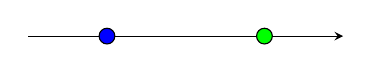
\begin{tikzpicture}[>=stealth]
    \draw[->](0,0)--(4,0);
    \filldraw[fill=blue] (1,0) circle[radius=0.1];
    \filldraw[fill=green] (3,0) circle[radius=0.1];
    \end{tikzpicture}
\end{center}
\begin{center}
    \begin{tikzpicture}[>=stealth]
    \draw[->](0,0)--(4,0);
    \draw[->](2,0.5)--(0,-1.5);
    \filldraw[fill=blue] (1,0) circle[radius=0.1];
    \filldraw[fill=green] (3,0) circle[radius=0.1];
    \end{tikzpicture}
\end{center}
\begin{center}
    \begin{tikzpicture}[>=stealth]
    \draw[->](0,0)--(4,0);
    \draw[->](2,0.5)--(0,-1.5);
    \draw[->](1.5,-0.8)--(1.5,2);
    \filldraw[fill=blue] (1,0) circle[radius=0.1];
    \filldraw[fill=green] (3,0) circle[radius=0.1];
    \end{tikzpicture}
\end{center}
\begin{itemize}
    \item 情報圧縮\\
    高次元空間上のデータを, 低次元の空間に, ある基準のもとで写像する
    \item 主成分分析\\
    低次元への写像に伴う情報のロスを最小に抑える線形写像
\end{itemize}
\subsection{主成分分析}
以下のように$R^{2}$の空間に分布するデータが与えられたとする.
\begin{center}
    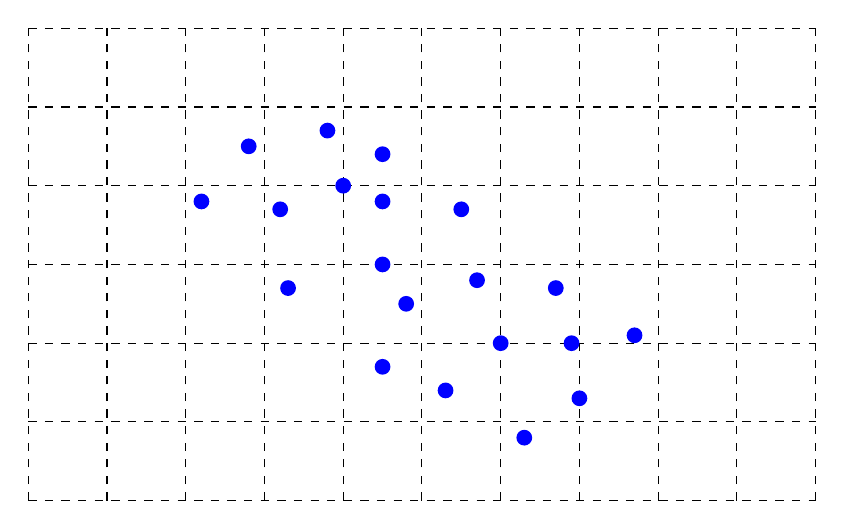
\begin{tikzpicture}
        \draw[dashed](0,0) grid (10,6);
        \fill[fill=blue](2.2,3.8) circle [radius=0.1];
        \fill[fill=blue](2.8,4.5) circle [radius=0.1];
        \fill[fill=blue](3.2,3.7) circle [radius=0.1];
        \fill[fill=blue](3.3,2.7) circle [radius=0.1];
        \fill[fill=blue](3.8,4.7) circle [radius=0.1];
        \fill[fill=blue](4,4) circle [radius=0.1];
        \fill[fill=blue](4.5,4.4) circle [radius=0.1];
        \fill[fill=blue](4.5,3.8) circle [radius=0.1];
        \fill[fill=blue](4.5,3) circle [radius=0.1];
        \fill[fill=blue](4.5,1.7) circle [radius=0.1];
        \fill[fill=blue](4.8,2.5) circle [radius=0.1];
        \fill[fill=blue](5.3,1.4) circle [radius=0.1];
        \fill[fill=blue](5.5,3.7) circle [radius=0.1];
        \fill[fill=blue](5.7,2.8) circle [radius=0.1];
        \fill[fill=blue](6,2) circle [radius=0.1];
        \fill[fill=blue](6.3,0.8) circle [radius=0.1];
        \fill[fill=blue](6.7,2.7) circle [radius=0.1];
        \fill[fill=blue](6.9,2) circle [radius=0.1];
        \fill[fill=blue](7,1.3) circle [radius=0.1];
        \fill[fill=blue](7.7,2.1) circle [radius=0.1];
    \end{tikzpicture}
\end{center}
この空間上に分布するデータを, 直線状の部分空間に写像することを考える. すると以下のような写像が考えられる.
\begin{center}
    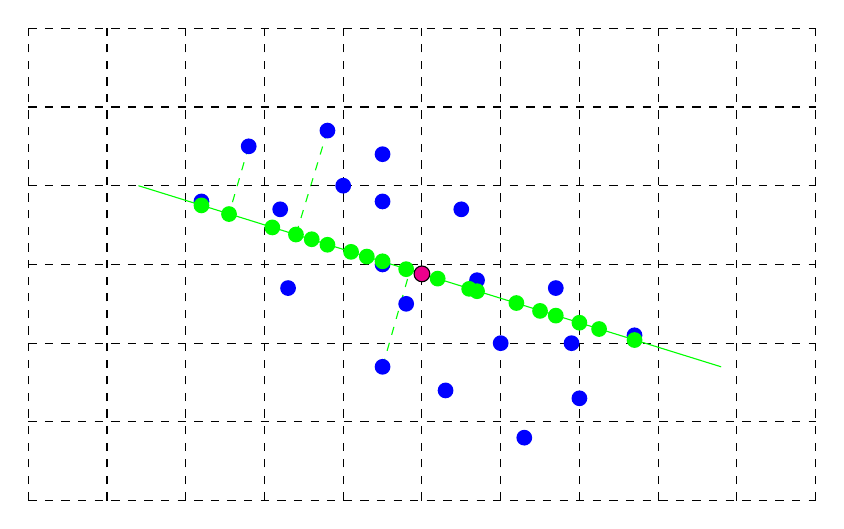
\begin{tikzpicture}
        \draw[draw=green,dashed] (2.8,4.5)--(2.55,3.64);
        \draw[draw=green,dashed] (3.8,4.7)--(3.4,3.38);
        \draw[draw=green,dashed] (4.5,1.7)--(4.85,2.93);
        \draw[dashed](0,0) grid (10,6);
        \fill[fill=blue](2.2,3.8) circle [radius=0.1];
        \fill[fill=blue](2.8,4.5) circle [radius=0.1];
        \fill[fill=blue](3.2,3.7) circle [radius=0.1];
        \fill[fill=blue](3.3,2.7) circle [radius=0.1];
        \fill[fill=blue](3.8,4.7) circle [radius=0.1];
        \fill[fill=blue](4,4) circle [radius=0.1];
        \fill[fill=blue](4.5,4.4) circle [radius=0.1];
        \fill[fill=blue](4.5,3.8) circle [radius=0.1];
        \fill[fill=blue](4.5,3) circle [radius=0.1];
        \fill[fill=blue](4.5,1.7) circle [radius=0.1];
        \fill[fill=blue](4.8,2.5) circle [radius=0.1];
        \fill[fill=blue](5.3,1.4) circle [radius=0.1];
        \fill[fill=blue](5.5,3.7) circle [radius=0.1];
        \fill[fill=blue](5.7,2.8) circle [radius=0.1];
        \fill[fill=blue](6,2) circle [radius=0.1];
        \fill[fill=blue](6.3,0.8) circle [radius=0.1];
        \fill[fill=blue](6.7,2.7) circle [radius=0.1];
        \fill[fill=blue](6.9,2) circle [radius=0.1];
        \fill[fill=blue](7,1.3) circle [radius=0.1];
        \fill[fill=blue](7.7,2.1) circle [radius=0.1];
        \draw[draw=green] (1.4,4)--(8.8,1.7);
        \fill[fill=green] (2.2,3.75) circle[radius=0.1];
        \fill[fill=green] (2.55,3.64) circle[radius=0.1];
        \fill[fill=green] (3.1,3.47) circle[radius=0.1];
        \fill[fill=green] (3.4,3.38) circle[radius=0.1];
        \fill[fill=green] (3.6,3.32) circle[radius=0.1];
        \fill[fill=green] (3.8,3.25) circle[radius=0.1];
        \fill[fill=green] (4.1,3.16) circle[radius=0.1];
        \fill[fill=green] (4.3,3.10) circle[radius=0.1];
        \fill[fill=green] (4.5,3.04) circle[radius=0.1];
        \fill[fill=green] (4.8,2.94) circle[radius=0.1];
        \fill[fill=green] (5.2,2.82) circle[radius=0.1];
        \fill[fill=green] (5.6,2.69) circle[radius=0.1];
        \fill[fill=green] (5.7,2.66) circle[radius=0.1];
        \fill[fill=green] (6.2,2.51) circle[radius=0.1];
        \fill[fill=green] (6.5,2.41) circle[radius=0.1];
        \fill[fill=green] (6.7,2.35) circle[radius=0.1];
        \fill[fill=green] (7,2.26) circle[radius=0.1];
        \fill[fill=green] (7.25,2.18) circle[radius=0.1];
        \fill[fill=green] (7.7,2.04) circle[radius=0.1];
        \filldraw[fill=magenta] (5,2.88) circle[radius=0.1];
    \end{tikzpicture}
\end{center}
\begin{center}
    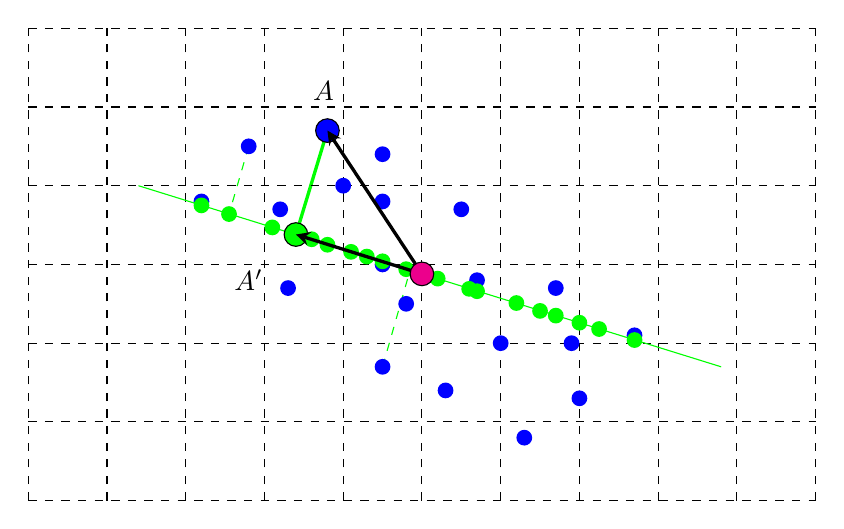
\begin{tikzpicture}[>=stealth]
        \draw[draw=green,dashed] (2.8,4.5)--(2.55,3.64);
        \draw[draw=green,very thick] (3.8,4.7)--(3.4,3.38);
        \draw[draw=green,dashed] (4.5,1.7)--(4.85,2.93);
        \draw[dashed](0,0) grid (10,6);
        \fill[fill=blue](2.2,3.8) circle [radius=0.1];
        \fill[fill=blue](2.8,4.5) circle [radius=0.1];
        \fill[fill=blue](3.2,3.7) circle [radius=0.1];
        \fill[fill=blue](3.3,2.7) circle [radius=0.1];
        \filldraw[fill=blue](3.8,4.7) circle [radius=0.15];
        \fill[fill=blue](4,4) circle [radius=0.1];
        \fill[fill=blue](4.5,4.4) circle [radius=0.1];
        \fill[fill=blue](4.5,3.8) circle [radius=0.1];
        \fill[fill=blue](4.5,3) circle [radius=0.1];
        \fill[fill=blue](4.5,1.7) circle [radius=0.1];
        \fill[fill=blue](4.8,2.5) circle [radius=0.1];
        \fill[fill=blue](5.3,1.4) circle [radius=0.1];
        \fill[fill=blue](5.5,3.7) circle [radius=0.1];
        \fill[fill=blue](5.7,2.8) circle [radius=0.1];
        \fill[fill=blue](6,2) circle [radius=0.1];
        \fill[fill=blue](6.3,0.8) circle [radius=0.1];
        \fill[fill=blue](6.7,2.7) circle [radius=0.1];
        \fill[fill=blue](6.9,2) circle [radius=0.1];
        \fill[fill=blue](7,1.3) circle [radius=0.1];
        \fill[fill=blue](7.7,2.1) circle [radius=0.1];
        \draw[draw=green] (1.4,4)--(8.8,1.7);
        \fill[fill=green] (2.2,3.75) circle[radius=0.1];
        \fill[fill=green] (2.55,3.64) circle[radius=0.1];
        \fill[fill=green] (3.1,3.47) circle[radius=0.1];
        \filldraw[fill=green] (3.4,3.38) circle[radius=0.15];
        \fill[fill=green] (3.6,3.32) circle[radius=0.1];
        \fill[fill=green] (3.8,3.25) circle[radius=0.1];
        \fill[fill=green] (4.1,3.16) circle[radius=0.1];
        \fill[fill=green] (4.3,3.10) circle[radius=0.1];
        \fill[fill=green] (4.5,3.04) circle[radius=0.1];
        \fill[fill=green] (4.8,2.94) circle[radius=0.1];
        \fill[fill=green] (5.2,2.82) circle[radius=0.1];
        \fill[fill=green] (5.6,2.69) circle[radius=0.1];
        \fill[fill=green] (5.7,2.66) circle[radius=0.1];
        \fill[fill=green] (6.2,2.51) circle[radius=0.1];
        \fill[fill=green] (6.5,2.41) circle[radius=0.1];
        \fill[fill=green] (6.7,2.35) circle[radius=0.1];
        \fill[fill=green] (7,2.26) circle[radius=0.1];
        \fill[fill=green] (7.25,2.18) circle[radius=0.1];
        \fill[fill=green] (7.7,2.04) circle[radius=0.1];
        \draw[very thick,->] (5,2.88)--(3.8,4.7);
        \draw[very thick,->] (5,2.88)--(3.4,3.38);
        \filldraw[fill=magenta] (5,2.88) circle[radius=0.15];
        \node at(2.8,2.8) {$A'$};
        \node at(3.75,5.2) {$A$};
    \end{tikzpicture}
\end{center}
このとき$A-A'$がロスとなる. $A'$において射影成分の分散が最大化されるように直線を引く時, これはロスが最小化されることとなる. これはOAの距離が一定であるので, $A-A'$の値が最小となるときは$O-A'$の値が最大となるためである.部分空間が変われば, 分散も変わるので, 最も射影成分の分散の大きくなる部分空間を求めることがよい. \\
次に第1主成分の求め方について扱う.\\
いま$P$次元のベクトルが,$N$個あるとする.
\begin{eqnarray*}
    \mbox{\boldmath $x$}_{n}=\begin{pmatrix}x_{np}\end{pmatrix},\ (p=1,2,3,\cdots,P)\ (n=1,2,3,\cdots,N)
\end{eqnarray*}
簡単のため, 各変数についてその平均値を0とする. 0ではない場合は平均値を引いて新たに変数を定義しなおせば一般性は失われない.\\
ここで, 測定データ全体は次の行列$X$で与えられる.
\begin{eqnarray*}
    X=\begin{pmatrix} \mbox{\boldmath $x$}_{1}&\mbox{\boldmath $x$}_{2}&\cdots&\mbox{\boldmath $x$}_{n}\end{pmatrix}^{T}=\begin{pmatrix} x_{11}&x_{12}&\cdots&x_{1P}\\ x_{21}&x_{22}&\cdots&x_{2P}\\\vdots&\vdots&\ddots&\vdots \\ x_{N1}&x_{N2}&\cdots&x_{NP} \end{pmatrix}
\end{eqnarray*}
求める主成分を
\begin{eqnarray*}
    \mbox{\boldmath $w$} = \begin{pmatrix}w_{1}&w_{2}&\cdots&w_{P}\end{pmatrix}^{T}\ \|\mbox{\boldmath $w$}\|=\mbox{\boldmath $w$}^{T}\mbox{\boldmath $w$}=1
\end{eqnarray*}
とし, 今$n$番目のデータを
\begin{eqnarray*}
    \mbox{\boldmath $x$}_{n}=\begin{pmatrix} x_{n1}&x_{n2}&\cdots&x_{nP}\end{pmatrix}^{T}
\end{eqnarray*}
の主成分への射影$z_{n}$を考えると,
\begin{eqnarray*}
    z_{n}=\mbox{\boldmath $x$}_{n}^{T}\mbox{\boldmath $w$}=\sum_{p=1}^{P}x_{np}w_{p}
\end{eqnarray*}
$\mbox{\boldmath $z$}=\begin{pmatrix}z_{1}&z_{2}&\cdots &z_{N}\end{pmatrix}^{T}$とすれば,
\begin{eqnarray*}
    \mbox{\boldmath $z$}=X\mbox{\boldmath $w$}
\end{eqnarray*}
このとき$z_{n}$の分散$\sigma^{2}$は
\begin{eqnarray*}
    \sigma^{2}&=&\frac{1}{N}\bm{z}^{T}\bm{z}=\frac{1}{N}(X\bm{w})^{T}(X\bm{w})\\
            &=&\frac{1}{N}\bm{w}^{T}X^{T}X\bm{w}=\bm{w}^{T}C\bm{w}
\end{eqnarray*}
ただし,
\begin{eqnarray*}
    C=\{c_{ij}\},\ c_{ij}=\frac{1}{N}\sum_{k=1}^{N}x_{ki}x_{kj}
\end{eqnarray*}
$C$は, 共分散行列とよばれ, 平均値が0でない一般的な場合は
\begin{eqnarray*}
    c_{ij}=\frac{1}{N}\sum_{k=1}^{N}(x_{ki}-{x_{i}})(x_{kj}-\bar{x_{j}})
\end{eqnarray*}
となる.\ ここで, 第1主成分は$\bm{w}$で$\sigma^{2}$の最大化すること. つまり
\begin{eqnarray*}
    \underset{\bm{w}}{\rm max}\bm{w}^{T}C\bm{w}
\end{eqnarray*}
を満たすことである. この中で条件として$\bm{w}^{T}\bm{w}=1$を満たさなければならない. 定式化すると
\begin{eqnarray*}
    \underset{\bm{w}}{\rm max}\bm{w}^{T}C\bm{w}\\
    s.t.\ \ \bm{w}^{T}\bm{w}=1
\end{eqnarray*}
\subsection{Lagrangeの未定乗数法}
以下の問題を求める方法である.
\begin{eqnarray*}
    \underset{x}{\rm max}f(\bm{x})\\
    s.t.\ g(\bm{x})=0
\end{eqnarray*}
一般的な解法として
\begin{align*}
   L(\bm{x})=f(\bm{x})+\lambda g(\bm{x}) \tag{6.1}
\end{align*}
とおき,
\begin{eqnarray*}
    \left\{
    \begin{array}{l}
      \displaystyle \frac{\partial}{\partial \bm{x}}L(\bm{x}) = 0\\
      g(\bm{x})=0
    \end{array}
    \right.
\end{eqnarray*}
の連立方程式を解くことである.\\
\begin{screen}
周囲の長さがXの長方形の中で, 面積の一番大きいものの辺の長さを求める.\\
各辺を$a,\,b$とおくと問題は
    \begin{eqnarray*}
        {\rm max}&& ab\\
        && s.t.\ 2(a+b)=X
    \end{eqnarray*}
    という問題となる.\\
    つまり, \\
    \begin{eqnarray*}
        f(a,b) &=& ab\\
        g(a,b) &=& 2(a+b)-X
    \end{eqnarray*}
    となるので,
    \begin{eqnarray*}
        L(a,b,\lambda) &=& f(a,b)- \lambda g(a,b)\\
                        &=& ab - \lambda (2a+2b-X)
    \end{eqnarray*}
    について連立方程式を立てて解けばよい.
    \begin{eqnarray*}
        && \frac{\partial}{\partial a} L (a,b,\lambda) = b-2\lambda = 0\\
        && \frac{\partial}{\partial b} L (a,b,\lambda) = a-2\lambda = 0\\
        && \frac{\partial}{\partial \lambda} L(a,b,\lambda) = -2a-2b+X = 0
    \end{eqnarray*}
    となるので, 整理すると
    \begin{eqnarray*}
        && a = b = \lambda\\
        && -4\lambda-4\lambda+X = 0\\
        && \lambda = \frac{X}{8}\\
        && a=b=2\lambda = \frac{X}{4}
    \end{eqnarray*}
となる.
\end{screen}
Lagrangeの未定乗数法を用いて$\bm{w}$による$\sigma^{2}$の最大化問題は$\|\bm{w}\|=\bm{w}^{T}\bm{w}=1$の条件の下で解くことを考える.\\
Lagrangeの未定乗数法より以下の方程式を立てる.
\begin{eqnarray*}
    L(\bm{w},\lambda)=\bm{w}^{T}C\bm{w}-\lambda(\bm{w}^{T}\bm{w}-1)
\end{eqnarray*}
とおいて, $\displaystyle \frac{\partial L}{\partial \bm{w}}=0$を解くことを考える. すると
\begin{eqnarray*}
    \frac{\partial L}{\partial \bm{w}}&=&C\bm{w}+(\bm{w}^{T}C)^{T}-\lambda(\bm{w}+\bm{w})\\
                                      &=&C\bm{w}+C^{T}\bm{w}-2\lambda \bm{w}\\
                                      &=&C\bm{w}+C\bm{w}-2\lambda \bm{w}\\
                                      &=&2(C-\lambda I)\bm{w} = 0
\end{eqnarray*}
となる. 共分散行列に関して
\begin{eqnarray*}
    c_{ij}=\frac{1}{N}\sum_{k=1}^{N}x_{ki}x_{kj} = \frac{1}{N}\sum_{k=1}^{N}x_{kj}x_{ki} = c_{ji}
\end{eqnarray*}
であるから, 対称行列であることがいえる. よって,
\begin{eqnarray*}
    (C-\lambda I)\bm{w} = 0 \ \Longleftrightarrow\ C\bm{w} = \lambda \bm{w}
\end{eqnarray*}
となり, 問題は固有値問題に帰着される.\\
また
\begin{eqnarray*}
    (C-\lambda I)\bm{w} = 0 \ \Longleftrightarrow\ {\rm det}|C-\lambda I|=0
\end{eqnarray*}
となるので, $\lambda$が満たすべき条件は, 共分散行列$C$の固有方程式となる.\\
したがって, 射影の分散の最大値を与える主成分$\bm{w}$は分散共分散行列の固有ベクトルのひとつであり, $\lambda$はその固有ベクトルに対応した固有値であることがわかる.\\
データ数が$P$個あることから$(C-\lambda I)\bm{w}=0$を満たす固有ベクトル$\bm{w}$, 固有値$\lambda$はそれぞれ$P$個ある.\\
このうち, どれが射影の分散の最大値を与えるかを考える.
\begin{eqnarray*}
    C\bm{w} = \lambda \bm{w}
\end{eqnarray*}
という関係の下,
\begin{eqnarray*}
    \sigma^{2}=\bm{w}^{T}C\bm{w}
\end{eqnarray*}
であるから
\begin{eqnarray*}
    \sigma^{2}=\bm{w}^{T}C\bm{w}=\lambda \bm{w}^{T}\bm{w}
\end{eqnarray*}
となり,\,$\bm{w}^{T}\bm{w}=1$であることを考慮すれば
\begin{eqnarray*}
    \sigma^{2}=\lambda
\end{eqnarray*}
となる. つまり\textcolor{red}{射影の分散の値は固有値に等しい}.\\
よって, 求める主成分は最大固有値に対応した固有ベクトルとして与えられることが分かる.\\[1cm]
第2以降の主成分の求め方について,\\
帰納的に第$m$主成分を求める. 分散共分散行列$C$の固有値のうち大きいものから順に$m-1$個に対応する固有ベクトルとして, $m-1$の主成分$\bm{w}_{1},\bm{w}_{2},\cdots ,\bm{w}_{k},\cdots,\bm{w}_{m-1}$が求まっているとする. これらのベクトルは
\begin{eqnarray*}
    &&(C-\lambda I)\bm{w}_{k}=0\\
    &&\bm{w}_{k}^{T}\bm{w}_{k}=1
\end{eqnarray*}
を満たし, 互いに直交しているものとする\footnote{$\bm{w}$は固有ベクトルなので自明}.
\begin{eqnarray*}
    \bm{w}_{k}^{T}\bm{w}_{k'(\neq k)}=0
\end{eqnarray*}
つまり
\begin{eqnarray*}
    f(\bm{w}_{m}) = \bm{w}_{m}^{T}C\bm{w}_{m}\\
    s.t.\ \bm{w}_{m}^{T}\bm{w}_{m}=1,\ \bm{w}_{k}^{T}\bm{w}_{k'(k'\neq k)}=0
\end{eqnarray*}
という関係式が得られる.\\
Lagrangeの未定乗数法より
\begin{align*}
    J_{m}=\bm{w}_{m}^{T}C\bm{w}_{m}-\lambda_{m}(\bm{w}_{m}^{T}\bm{w}_{m}-1)-\sum_{k=1}^{m-1}\mu_{k}\bm{w}_{m}^{T}\bm{w}_{k}
\end{align*}
とおいて, $\displaystyle \frac{\partial J_{m}}{\partial \bm{w}_{m}}=0$とおくと,
\begin{eqnarray*}
    &&2C_{\bm{w}_{m}}-2\lambda_{m}\bm{w}-\sum_{k=1}^{m-1}\mu_{k}\bm{w}_{k}=0\\
   \Longleftrightarrow\ && C_{\bm{w}}-\lambda_{m}\bm{w}_{m}-\sum_{k=1}^{m-1}\mu_{k}\bm{w}_{k}=0 
\end{eqnarray*}
ここで$\mu_{k}$について$\mu_{k}=\frac{1}{2}\mu_{k}$として再定義.\\
左から$\bm{w}_{j}^{T}\,(j=1,2,3,\cdots,m-1)$をかけると,($\bm{w}_{k}^{T}\bm{w}_{k'(k' \neq k)}=0$を考慮して)
\begin{eqnarray*}
&&\bm{w}_{j}^{T}C\bm{w}_{m}-\lambda_{m}\bm{w}_{j}^{T}\bm{w}_{m}-\sum_{k=1}^{m-1}\mu_{k}\bm{w}_{j}\bm{w}_{k}=0\\
    \Longleftrightarrow \ && \bm{w}_{j}^{T}C\bm{w}_{m}-\mu_{j}=0
\end{eqnarray*}
となる. また
\begin{eqnarray*}
    \bm{w}_{j}^{T}C\bm{w}_{m}&=&\bm{w}_{m}^{T}C\bm{w}_{j}\\
                             &=&\lambda_{j}\bm{w}_{m}^{T}\bm{w}_{j}=0\ (j=1,2,\cdots,m-1) 
\end{eqnarray*}
であることから
\begin{eqnarray*}
    \mu_{j}=0\ (j=1,2,\cdots,m-1)
\end{eqnarray*}
となる. これから最適化のための評価関数として以下の関係式が導かれる.
\begin{align*}
    J_{m}=\bm{w}_{m}^{T}C\bm{w}_{m}\lambda_{m}(\bm{w}_{m}^{T}\bm{w}_{m}-1) \tag{6.2}
\end{align*}
よって, 第1主成分を求めるための評価関数と同じであるから, 求める第$m$主成分$\bm{w}_{m}$は\textcolor{red}{分散共分散行列の$C$の$m$番目に大きい固有値に対応した固有ベクトルとして与えられる}.\\[1cm]
\begin{itemize}
  \item 寄与率\ :\ 部分空間で表現出来る分布の広がり程度\\
    -元の空間における分散\ :\ $\sigma_{O}^{2}$\\
    -第$m$時の部分空間における分散\ :\ $\sigma_{Sm}^{2}$\\
    とすると
    \begin{align*}
      寄与率=\frac{\sigma_{Sm}^{2}}{\sigma_{O}^{2}} \tag{6.3}
    \end{align*}
    となる.
  \item 累積寄与率
    \begin{align*}
      累積寄与率=\frac{\sum_{m=1}^{M}\sigma_{Sm}^{2}}{\sigma_{O}^{2}} \tag{6.4}
    \end{align*}
\end{itemize}
\subsection{線形判別分析(LDA:Linear Discriminant Analysis}
級内分散$C_{W}$と級間分散$C_{B}$の比を最大にする座標空間を求める.
\begin{center}
    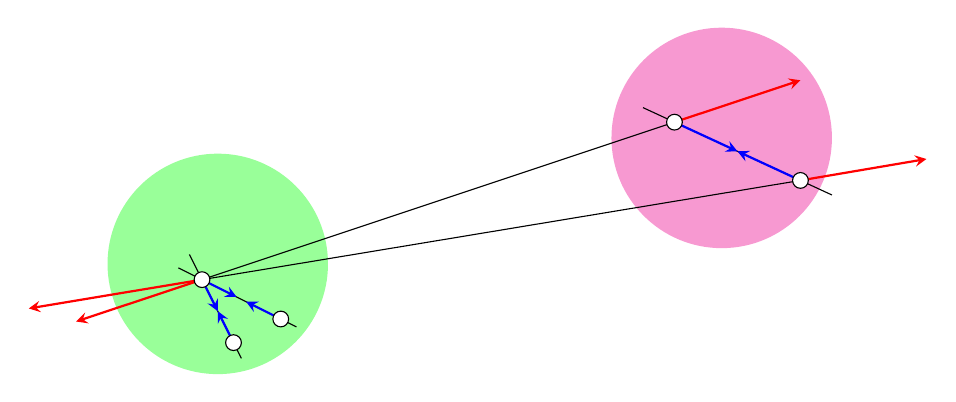
\begin{tikzpicture}[>=stealth,scale=2]
        \fill[fill=green!40] (0.1,0.1) circle[radius=0.7];
        \fill[fill=magenta!40] (3.3,0.9) circle[radius=0.7];
        \draw(0,0)--(3,1);
        \draw(0,0)--(3.8,0.63);
        \draw[thick,red,->] (0,0)--(-0.8,-0.266);
        \draw[thick,red,->] (0,0)--(-1.1,-0.183);
        \draw[thick,red,->] (3,1)--(3.8,1.266);
        \draw[thick,red,->] (3.8,0.63)--(4.6,0.766);
        \draw (-0.15,0.075)--(0.6,-0.3);
        \draw (-0.08,0.16)--(0.25,-0.5);
        \draw[->,draw=blue,thick] (0,0)--(0.1,-0.2);
        \draw[->,draw=blue,thick] (0.2,-0.4)--(0.1,-0.2);
        \draw[->,draw=blue,thick] (0,0)--(0.22,-0.11);
        \draw[->,draw=blue,thick](0.5,-0.25)--(0.28,-0.14);
        \draw (2.8,1.0925)--(4,0.5375);
        \draw[->,draw=blue,thick] (3,1)--(3.4,0.815);
        \draw[->,draw=blue,thick] (3.8,0.63)--(3.4,0.815);
        \filldraw[fill=white] (0,0) circle[radius=0.05];
        \filldraw[fill=white] (3,1) circle[radius=0.05];
        \filldraw[fill=white] (3.8,0.63) circle[radius=0.05]; 
        \filldraw[fill=white] (0.2,-0.4) circle[radius=0.05];
        \filldraw[fill=white] (0.5,-0.25) circle[radius=0.05];
    \end{tikzpicture}
\end{center}
カテゴリの同じデータは近くに, 違うデータは遠くに配置する.\\
2クラスの場合のLDAについて考えてみる. 2クラスについてそれぞれクラス$A,\,B$として以下の関数について考えてみる.\\
$y=\bm{w}^{T}\bm{x}$\\
$\mu'=E[y],\ \sigma'=E[(y-\mu)^{2}]$\\
として
\begin{eqnarray*}
    J(\bm{w})=\frac{(\mu_{A}'-\mu_{B}')^{2}}{\sigma_{A}'^{2}+\sigma_{B}'^{2}}
\end{eqnarray*}
射影ベクトル$\bm{w}$を変えると$J$の値が変わると, $J$が大きい時, 違うデータの集まりが遠くに配置されていることになるので, 識別が容易になる.\ したがって, $J$を最大化するベクトル$\bm{w}$を求めることでクラスを分割することができる.\\
$\bm{x}$\ :\ 特徴ベクトル\\
$n_{i}$\ :\ クラス$i$のデータ数$\displaystyle \left(総データ数 n=\sum_{i}n_{i}\right)$\\
$\bm{\mu}_{i}$\ :\ クラス$i$の平均ベクトル\\
$X_{i}$\ :\ クラス$i$に対する元空間における特徴ベクトルの集合\\
とおくと,
$C_{i}$\ :\ クラス$i$の共分散行列\\
$S_{i}$\ :\ クラス$i$の変動行列\\
は次式で定義される.
\begin{eqnarray*}
    C_{i}&=&\frac{1}{n_{i}}\sum_{\bm{x}\in X_{i}}(\bm{x}-\bm{\mu}_{i})(\bm{x}-\bm{\mu}_{i})^{T}\\
    S_{i}&=&\sum_{\bm{x}\in X_{i}}(\bm{x}-\bm{\mu}_{i})(\bm{x}-\bm{\mu}_{i})^{T}=n_{i}C_{i}
\end{eqnarray*}
また, 射影先について考える.ベクトル$\bm{w}$に$\bm{x}$を射影して作った1次元の空間において\\
$y$\ :\ 射影して作られた$\bm{x}$の像\ $y=\bm{w}^{T}\bm{x}$\\
$\tilde{\mu_{i}}$\  :\ 射影先の空間におけるクラス$i$のデータの平均値\\
$Y_{i}$\ :\ 射影先の空間におけるクラス$i$のデータの集合\\
$\tilde{\sigma_{i}}^{2}$\ :\ 射影先の空間におけるクラス$i$のデータの分散\\
$\tilde{S}_{i}$\ :\ 射影先の空間におけるクラス$i$の変動(行列)\\
とすると
\begin{eqnarray*}
    \tilde{\sigma}_{i}^{2}&=&\frac{1}{n_{i}}\sum_{y\in Y_{i}}(y-\tilde{\mu_{i}})^{2}\\
                          &=&\frac{1}{n_{i}}\sum_{x\in X_{i}}\|\bm{x}-\bm{\mu}_{i}\|^{2}\\
                          &=&\frac{1}{n_{i}}\sum_{x\in X_{i}}(\bm{w}^{T}\bm{x}-\bm{w}^{T}\bm{\mu}_{i})(\bm{w}^{T}\bm{x}-\bm{w}^{T}\bm{\mu}_{i})^{T}\\
                          &=&\frac{1}{n_{i}}\sum_{x\in X_{i}}\bm{w}(\bm{x}-\bm{\mu}_{i})(\bm{x}-\bm{\mu}_{i})^{T}\bm{w}\\
                          &=&\bm{w}^{T}C_{i}\bm{w}
\end{eqnarray*}
また, クラス$i$の変動については
\begin{eqnarray*}
    \tilde{S}_{i}=\sum_{y\in Y_{i}}(y-\tilde{\mu}_{i})^{2}=n_{i}\sigma_{i}^{2}=n_{i}\bm{w}^{T}C_{i}\bm{w}
\end{eqnarray*}
となる.クラス内変動$S_{w}$およびクラス間変動$S_{B}$を以下のように定義.
\begin{eqnarray*}
    S_{W}&=&S_{1}+S_{2}=\sum_{i=1,2}\sum{x\in X_{i}}(\bm{x}-\bm{\mu}_{i})(\bm{x}-\bm{\mu}_{i})^{T}\\
    S_{B}&=&\sum_{i=1,2}n_{i}(\bm{\mu}_{i}-\bm{\mu})(\bm{\mu}_{i}-\bm{\mu})^{T}
\end{eqnarray*}
ただし, $\mu$は全データの平均値であり, このときの射影先におけるクラス内変動$\tilde{S}_{W}$, クラス間変動$\tilde{S}_{B}$は以下のようになる.
\begin{eqnarray*}
    \tilde{S}_{W}&=&\tilde{S}_{1}+\tilde{S}_{2}=\bm{w}^{T}S_{W}\bm{w}\\
    \tilde{S}_{B}&=&\sum_{i=1,2}n_{i}(\tilde{\mu}_{i}-\tilde{\mu})^{2}\\
                 &=&n_{1}\left(\tilde{\mu}_{1}-\frac{n_{1}\tilde{\mu}_{1}+n_{2}\tilde{\mu}_{2}}{n}\right)^{2}+n_{2}\left(\tilde{\mu}_{2}-\frac{n_{1}\tilde{\mu}_{1}+n_{2}\tilde{\mu}_{2}}{n}\right)^{2}\\
                 &=&n_{1}\left(\frac{n_{2}(\tilde{\mu}_{1}-\tilde{\mu}_{2})}{n}\right)^{2}+n_{2}\left(\frac{n_{1}(\tilde{\mu}_{1}-\tilde{\mu}_{2})}{n}\right)^{2}\\
                 &=&\left(\frac{n_{1}n_{2}^{2}}{n^{2}}+\frac{n_{1}^{2}n_{2}}{n^{2}}\right)(\tilde{\mu}_{1}-\tilde{\mu}_{2})^{2}\\
                 &=&\frac{n_{1}n_{2}}{n}(\tilde{\mu}_{1}-\tilde{\mu}_{2})^{2}\\
                 &=&\bm{w}^{T}S_{B}\bm{w}
\end{eqnarray*}
$J$を以下のように定義.
\begin{align*}
    J=\frac{\tilde{S}_{B}}{\tilde{S}_{W}}=\frac{n_{1}n_{2}}{n}\cdot \frac{(\tilde{\mu}_{1}-\tilde{\mu}_{2})^{2}}{n_{1}\tilde{\sigma}_{1}^{2}+n_{2}\tilde{\sigma}_{2}^{2}} \tag{6.5}
\end{align*}
これより先の計算結果から以下の式が得られる.
\begin{eqnarray*}
    J=\frac{\bm{w}^{T}S_{B}\bm{w}}{\bm{w}^{T}S_{W}\bm{w}}
\end{eqnarray*}
この$J$を最大にする$\bm{w}$を求める問題を解く. また制約条件として
\begin{eqnarray*}
    \bm{w}^{T}S_{W}\bm{w}=1
\end{eqnarray*}
と定めるとき,
\begin{eqnarray*}
    \bm{w}^{T}S_{B}\bm{w}
\end{eqnarray*}
を最大にする問題と等価である.
ここでLagrangeの未定乗数法と同様にして以下のように$E$を定義する.
\begin{eqnarray*}
    E=\bm{w}^{T}S_{B}\bm{w}-\lambda(\bm{w}^{T}S_{W}\bm{w}-1)
\end{eqnarray*}
これに$\bm{w}$で偏微分してゼロとおくと,
\begin{eqnarray*}
    &&S_{B}\bm{w}-\lambda S_{W}\bm{w}=0\\
    \Longleftrightarrow\ && S_{W}^{-1}S_{B}\bm{w}-\lambda S_{W}^{-1}S_{W}\bm{w}=0\\
    \Longleftrightarrow\ && (S_{W}^{-1}S_{B}-\lambda I)\bm{w}=0
\end{eqnarray*}
となる.\\
したがって, $S_{W}^{-1}S_{B}$の固有値を求めればよいということがわかる. つまり$S_{W}^{-1}S_{B}$の最大固有値を$\lambda_{1}$とすれば, $J$の最大値を与える$\bm{w}$は$\lambda_{1}$に対する固有ベクトルとして求めることができる.\\[1cm]
多クラスの場合のLDAについて$N$クラスの問題は$N-1$軸に射影することを考える.\\
ベクトル$\bm{w}_{i}\ (i=1,\cdots,N-1)$に$\bm{x}$を射影して作った$N-1$次元の空間において\\
$\bm{y}$\ :\ 射影して作られた$\bm{x}$の像\ $\bm{y}=W^{T}\bm{x},\ W=\begin{pmatrix}\bm{w}_{1}&\bm{w}_{2}&\cdots&\bm{w}_{N-1}\end{pmatrix}$\\
$\tilde{\mu}_{i}$\ :\ 射影先の空間におけるクラス$i$のデータの平均値\\
$Y_{i}$\ :\ 射影先の空間におけるクラス$i$のデータの集合\\
$\tilde{C}_{i}$\ :\ 射影先の空間におけるクラス$i$のデータの共分散行列\\
$\tilde{S}_{i}$\ :\ 射影先の空間におけるクラス$i$の変動行列\\
とすると
\begin{eqnarray*}
    \tilde{C}_{i}&=&\frac{1}{n_{i}}\sum_{y\in Y_{i}}(\bm{y}-\tilde{\bm{\mu}}_{i})(\bm{y}-\tilde{\bm{\mu}}_{i})^{T}\\
                 &=&\frac{1}{n_{i}}\sum_{x\in X_{i}}\bm{w}^{T}(\bm{x}-\bm{mu}_{i})(\bm{x}-\bm{mu}_{i})^{T}\bm{w}=\bm{w}^{T}C_{i}\bm{w}
\end{eqnarray*}
2クラスのときと同様に
\begin{eqnarray*}
    S_{W}&=&\sum_{i=1}^{N}S_{i}=\sum_{i=1}^{N}\sum_{\bm{x}\in X_{i}}(\bm{x}-\bm{\mu}_{i})(\bm{x}-\bm{\mu}_{i})^{T}=\sum_{i=1}^{N}n_{i}C_{i}\\
    S_{B}&=&\sum_{i=1}^{N}n_{i}(\bm{\mu}_{i}-\bm{\mu})(\bm{\mu}_{i}-\bm{\mu})^{T}
\end{eqnarray*}
また,
\begin{eqnarray*}
    C_{W}&=&\frac{1}{n}S_{W},\ C_{B}=\frac{1}{n}S_{B}\\
    \tilde{C}_{W}=W^{T}C_{W}W,\ \tilde{C}_{B}=W^{T}C_{B}W
\end{eqnarray*}
これの$\tilde{C_{B}}$と$\tilde{C}_{W}$の比が大きくなるように$W$を設定すればよい.\\
2クラスのときと異なり,\ $\tilde{C}_{B},\ \tilde{C}_{W}$は行列であるから, 単純な比を取る代わりに, (例えば)次の$J$を評価関数と取る.
\begin{eqnarray*}
    J=\frac{{\rm tr}\tilde{C}_{B}}{{\rm tr}\tilde{C}_{W}}
\end{eqnarray*}
ここで, tr(トレース)とは, 行列の対角成分の和のことである.\\
この関数の$W$による最大化は
\begin{eqnarray*}
    W^{T}C_{W}W=I
\end{eqnarray*}
となる条件で, 分子を最大化することと等価である.\ つまり以下の評価関数の最大化問題である.
\begin{eqnarray*}
    E=\sum_{i=1}^{N-1}\bm{w}_{i}^{T}C_{B}\bm{w}_{i}-\sum_{i=1}^{N-1}\lambda_{i}(\bm{w}_{i}^{T}C_{W}\bm{w}_{i}-1)
\end{eqnarray*}
$\bm{w_{i}}$で偏微分してゼロとしておくと
\begin{eqnarray*}
    &&C_{B}\bm{w}_{i}-\lambda_{i}C_{W}\bm{w}_{i}=0\\
    \Longleftrightarrow && C_{W}^{-1}C_{B}\bm{w}_{i}-\lambda_{i}C_{W}^{-1}C_{W}\bm{w}_{i}=0\\
    \Longleftrightarrow && (C_{W}^{-1}C_{B}-\lambda_{i}I)\bm{w}_{i}=0
\end{eqnarray*}
をえるので, 問題は$C_{W}^{-1}C_{B}$の固有値を求める問題に帰着する.\\
つまり, $C_{W}^{-1}C_{B}$の固有値の大きい方から$N-1$個とって, これらに対応する固有ベクトル$\bm{w}_{i},\ (i=1,2,\cdots,N-1)$を求めれば, これが$W$の各列ベクトルとなる.\\
データ間の距離と分散の関係は以下のようになる.
\begin{eqnarray*}
    \sum_{i=1}^{N}\sum_{j=i+1}^{N}(x_{i}-x_{j})^{2}&=& \sum_{i=1}^{N}\sum_{j=i+1}^{N}(x_{i}^{2}-2x_{i}x_{j}+x_{j}^{2})\\
                                                   &=& (N-1)\sum_{i=1}^{N}x_{i}^{2}-2\sum_{i=1}^{N}\sum_{j=i+1}^{N}x_{i}x_{j}\\
                                                   &=& N\sum_{i=1}^{N}x_{i}^{2}-\left(\sum_{i=1}^{N}x_{i}^{2}+2\sum_{i=1}^{N}\sum_{j=i+1}^{N}x_{i}x_{j}\right)\\
                                                   &=& N\sum_{i=1}^{N}x_{i}^{2}-\left(\sum_{i=1}^{N}x_{i}\right)^{2}\\
                                                   &=& N^{2}\left(\frac{1}{N}\sum_{i=1}^{N}x_{i}^{2}-\left(\frac{1}{N}\sum_{i=1}^{N}x_{i}\right)^{2}\right)\\
                                                   &=& N\sum_{i=1}^{N}(x_{i}-\bar{x})^{2}
\end{eqnarray*}
Pair-wiseの距離について\\
$z_{i}=\bm{x}_{i}^{T}\bm{a}$\\
として
\begin{eqnarray*}
    E&=&\frac{1}{2}\sum_{i=1}^{N}\sum_{j=1}^{N}(z_{i}-z_{j})^{2}=\frac{1}{2}\sum_{i=1}^{N}\sum_{j=1}^{N}\bm{a}^{T}(\bm{x}_{i}-\bm{x}_{j})(\bm{x}_{i}-\bm{x}_{j})^{T}\bm{a}\\
     &=&\frac{1}{2}\bm{a}^{T}\left(\sum_{i=1}^{N}\sum_{j=1}^{N}(\bm{x}_{i}-\bm{x}_{j})(\bm{x}_{i}-\bm{x}_{j})^{T}\right)\bm{a}\\
     &=&\bm{a}^{T}\left(N\sum_{i=1}^{N}\bm{x}_{i}\bm{x}_{i}^{T}\right)\bm{a}-\bm{a}^{T}\left(\sum_{i=1}^{N}\sum_{j=1}^{N}\bm{x}_{j}\bm{x}_{i}^{T}\right)\bm{a}\\
     &=&\bm{a}^{T}\left(N\sum_{i=1}^{N}\bm{x}_{i}\bm{x}_{i}^{T}\right)\bm{a}-\bm{a}^{T}\left(\sum_{i=1}^{N}\sum_{j=1}^{N}\bm{x}_{j}\bm{x}_{i}^{T}\right)\bm{a}\\
     &=&\bm{a}^{T}XBX^{T}\bm{a}-\bm{a}^{T}XX^{T}\bm{a}\\
     &=&\bm{a}^{T}XCX^{T}\bm{a}
\end{eqnarray*}
であり
\begin{eqnarray*}
    X=\begin{pmatrix} \bm{x}_{1}&\bm{x}_{2}&\cdots&\bm{x}_{N}\end{pmatrix},\ B=\begin{pmatrix}b_{ij}\end{pmatrix}\ b_{ij}=\left\{ \begin{array}{l} N\ \ i=j\\ 0\ \ i\neq j \end{array} \right. \ C=B-I
\end{eqnarray*}
つまり, 主成分分析は, 上記$XCX^{T}$の最大固有値に対する, 固有ベクトルを求める問題である.\\[1cm]
$i,j$で決まる重み$w_{ij}$を導入する.
\begin{eqnarray*}
    E&=&\frac{1}{2}\sum_{i=1}^{N}\sum_{j=1}^{N}w_{ij}(z_{i}-z_{j})^{2}=\frac{1}{2}\sum_{i=1}^{N}\sum_{j=1}^{N}\bm{a}^{T}(\bm{x}_{i}-\bm{x}_{j})w_{ij}(\bm{x}_{i}-\bm{x}_{j})^{T}\bm{a}\\
     &=&\bm{a}^{T}\left(\sum_{i=1}^{N}\sum_{j=1}^{N}\bm{x}_{i}w_{ij}\bm{x}_{i}^{T}\right)\bm{a}-\bm{a}^{T}\left(\sum_{i=1}^{N}\sum_{j=1}^{N}\bm{x}_{i}w_{ij}\bm{x}_{j}^{T}\right)\bm{a}\\
     &=&\bm{a}^{T}XDX^{T}\bm{a}-\bm{a}^{T}XWX^{T}\bm{a}=\bm{a}^{T}XLX^{T}\bm{a}\\
    D&=&\begin{pmatrix}d_{ij}\end{pmatrix},\ d_{ij}=\left\{ \begin{array}{l} \displaystyle \sum_{k=1}^{N}w_{ik}\ \ i=j\\ 0\ \ i\neq j \end{array} \right. W=\begin{pmatrix}w_{ij} \end{pmatrix} \ L=D-W\\
    F&=&\frac{\bm{a}^{T}XLX^{T}\bm{a}}{\bm{a}^{T}XDX^{T}\bm{a}}
\end{eqnarray*}
ここで
\begin{eqnarray*}
    w_{ij}={\rm exp}\left(-\frac{\|\bm{x}_{i}-\bm{x}_{j}\|}{t}\right)
\end{eqnarray*}
のように, $w_{ij}$を$\bm{x}_{i}$と$\bm{x}_{j}$との距離が大きいときに小さく, 距離が小さいときに1をとって, $F$を最小化することで, つまり$(XDX^{T})^{-1}XLX^{T}$の最小固有値に対する固有ベクトルとして$\bm{a}$を定めれば, 変換前の座標系で近くに分布しているデータ同士の写像後の距離を小さくすることが出来る.\\
$\Rightarrow$ Locality Preserving Projection\\[1cm]
重みつき分散の比の導入について
\begin{eqnarray*}
    E&=&\frac{\displaystyle \sum_{i=1}^{N}\sum_{j=i+1}^{N}w_{ij}(z_{i}-z_{j})^{2}}{\displaystyle \sum_{i=1}^{N}\sum_{j=i+1}^{N}v_{ij}(z_{i}-z_{j})^{2}}\\
     &=&\frac{\displaystyle \sum_{i=1}^{N}\sum_{j=1}^{N}\bm{a}^{T}(\bm{x}_{i}-\bm{x}_{j})w_{ij}(\bm{x}_{i}-\bm{x}_{j})^{T}\bm{a}}{\displaystyle \sum_{i=1}^{N}\sum_{j=1}^{N}\bm{a}^{T}(\bm{x}_{i}-\bm{x}_{j})v_{ij}(\bm{x}_{i}-\bm{x}_{j})^{T}\bm{a}}\\
     &=&\frac{\bm{a}^{T}XDX^{T}\bm{a}-\bm{a}^{T}XWX^{T}\bm{a}}{\bm{a}^{T}XGX^{T}\bm{a}-\bm{a}^{T}-\bm{a}^{T}XVX^{T}\bm{a}}\\
     &=&\frac{\bm{a}^{T}XLX^{T}\bm{a}}{\bm{a}^{T}XMX^{T}\bm{a}}
\end{eqnarray*}
とし,
\begin{eqnarray*}
    &&G_{ij}=\begin{pmatrix}g_{ij}\end{pmatrix}\ \ g_{ij}=\left\{ \begin{array}{l} \displaystyle \sum_{k=1}^{N}v_{ik}\ \ i=j\\ 0\ \ i\neq j \end{array} \right.\\
    &&V_{ij}=\begin{pmatrix}v_{ij}\end{pmatrix}\\
    &&M=G-V
\end{eqnarray*}
ここで,
\begin{eqnarray*}
    w_{ij}=\left\{ \begin{array}{l} 1 \ \bm{x}_{i}と\bm{x}_{j}が違うクラス\\ 0\ \ \bm{x}_{i}と\bm{x}_{j}が同じクラス\end{array} \right.\\
    v_{ij}=\left\{ \begin{array}{l} 1 \ \bm{x}_{i}と\bm{x}_{j}が違うクラス\\ 0\ \ \bm{x}_{i}と\bm{x}_{j}が同じクラス\end{array} \right.   
\end{eqnarray*}
として, $E$を最大化すれば, $LDA$と等価である.
\subsection{重み付き分散比とCDDA(クラス間距離を考慮した判別分析)}
いくつかの多クラスの問題では, \textcolor{red}{クラス間の距離に応じて, データを分布させたいことがある}\\
例えば, 年齢分布の30歳のカテゴリの横に31歳のカテゴリを分布させたいなどである.
\begin{center}
    \begin{tikzpicture}
      \draw(0,5)--(0,0)--(8,0);
      \draw[draw=blue,very thick] (0,4) to[out=0,in=135] (3,2) to[out=-45,in=178] (8,0);
      \draw[draw=red,very thick] (0,0) to[out=2,in=225] (3,2) to[out=45,in=182] (8,4);
      \node at(-0.5,2.5) {\rotatebox{90}{重みの大きさ}};
      \node at(8,-0.5) {クラス間の距離};
      \node at(7.6,0.5) {$v_{ij}$};
      \node at(7.6,4.5) {$w_{ij}$};
    \end{tikzpicture}
\end{center}
CDDA\ :\ Class Distance-based Discriminant Analysis\\
クラスが遠いデータは離れようとする. ただし, 十分離れていれば差はつけないというものである.\\
クラスが近いデータは近づこうとする. ただし, 十分近いデータは差をつけないというものである.
